\documentclass[10.5pt]{article} % Defines the document class
\usepackage{xeCJK}
% Package inclusions go here
\usepackage[utf8]{inputenc} % For UTF-8 encoding
\usepackage[T1]{fontenc} % T1 Font encoding
\usepackage{lmodern} % Modern LaTeX fonts
\usepackage{graphicx} % To include images
\usepackage{indentfirst} % Indent first paragraph after section title
\usepackage{lipsum} % For generating filler text
\usepackage[left=2cm,right=2cm,top=1cm,bottom=2cm]{geometry} % Page margins
\linespread{1.25}
\usepackage{pdfpages}
\title{科研成果认定说明} % Document title
\author{高丁超} % Author name
\date{} % Date
\pagestyle{empty}
\begin{document}

\maketitle % Generates the title
\thispagestyle{empty}
\section*{尊敬的各位老师:} % An unnumbered section

本人于2021年9月进入软件所计算机科学国家重点实验室开始硕士研究生的学习,导师为应圣钢副研究员,主要研究方向是量子计算机。我将申请参加2024年夏季硕士学位论文答辩。
本文将介绍我在硕士学习阶段所完成的研究工作,以及研究成果中本人的具体贡献。
从而方便各位老师了解本人的科研工作,并给出认定。


\paragraph*{研究成果简介:} % Numbered section
在硕士研究期间,本人主要参与了基于TDD的量子模型检测工具的开发。TDD是一种针对量子计算机优化的数据结构,在表示量子线路的张量网络上有显著优势。
量子模型检测是一种自动化验证量子系统是否满足特定命题的方法。随着量子系统中量子比特的增加,量子模型检测存在资源爆炸的缺点。
使用TDD作为量子模型检测的基础,可以显著降低量子模型检测中的资源消耗。

\paragraph*{研究成果贡献说明:}在应用TDD进行量子模型检测的工具开发过程中,本人主要参与了对TDD结构进行拆分,从而进一步优化量子模型检测执行效率的方案设计与python代码实现。
同时本人负责所有不同优化方案的对比实验设计与python代码实现。
后续工作中,本人也参与了C++语言版本中,TDD结构的实现,以及进一步改进LimTDD的C++ 版本实现。

\paragraph*{研究成果投稿情况:}
基于TDD的量子模型检测的科研工作,已将研究成果总结为一篇论文。其中本人作为第二作者。
该成果开始是投了CCF-B的ICCAD,结果是拒稿。五分制下,三位审稿人的评分分别是2,4,4。具体意见可见附录一。
后来这篇论文投了CCF-A的DAC,结果是 Work-in-Progress (WIP) poster sessions at the 61th DAC,也就是只展示海报。五分制下四位审稿人的评分都是3。具体意见可见附录二。

% Concluding remarks
% Another unnumbered section
\paragraph*{}
\setlength{\parindent}{0pt}
综上所述,本人在硕士研究期间所完成的工作有一定科研价值。诚挚希望各位老师能够对我的研究成果给予\textbf{2分认定}。\\[0.5cm]
% \noindent 申请人签字:
% \hfill[5cm]% Space for signature
% 导师签字:\\[1.5cm]
% \noindent
\begin{tabular}{p{0.4\linewidth} p{0.4\linewidth}}
    申请人签字: & \centering 导师签字: \\
\end{tabular}
\section*{专家评价意见}
\setlength{\parindent}{0pt}

专家一意见:\\[1.2cm]
专家二意见:\\[1.2cm]
专家三意见:\\[1.2cm]
% \begin{tabular}{p{0.4\linewidth} p{0.4\linewidth}}
%     专家一意见: & \centering 专家二意见:\\
%     专家三意见: & \\
% \end{tabular}
\newpage
\thispagestyle{empty}

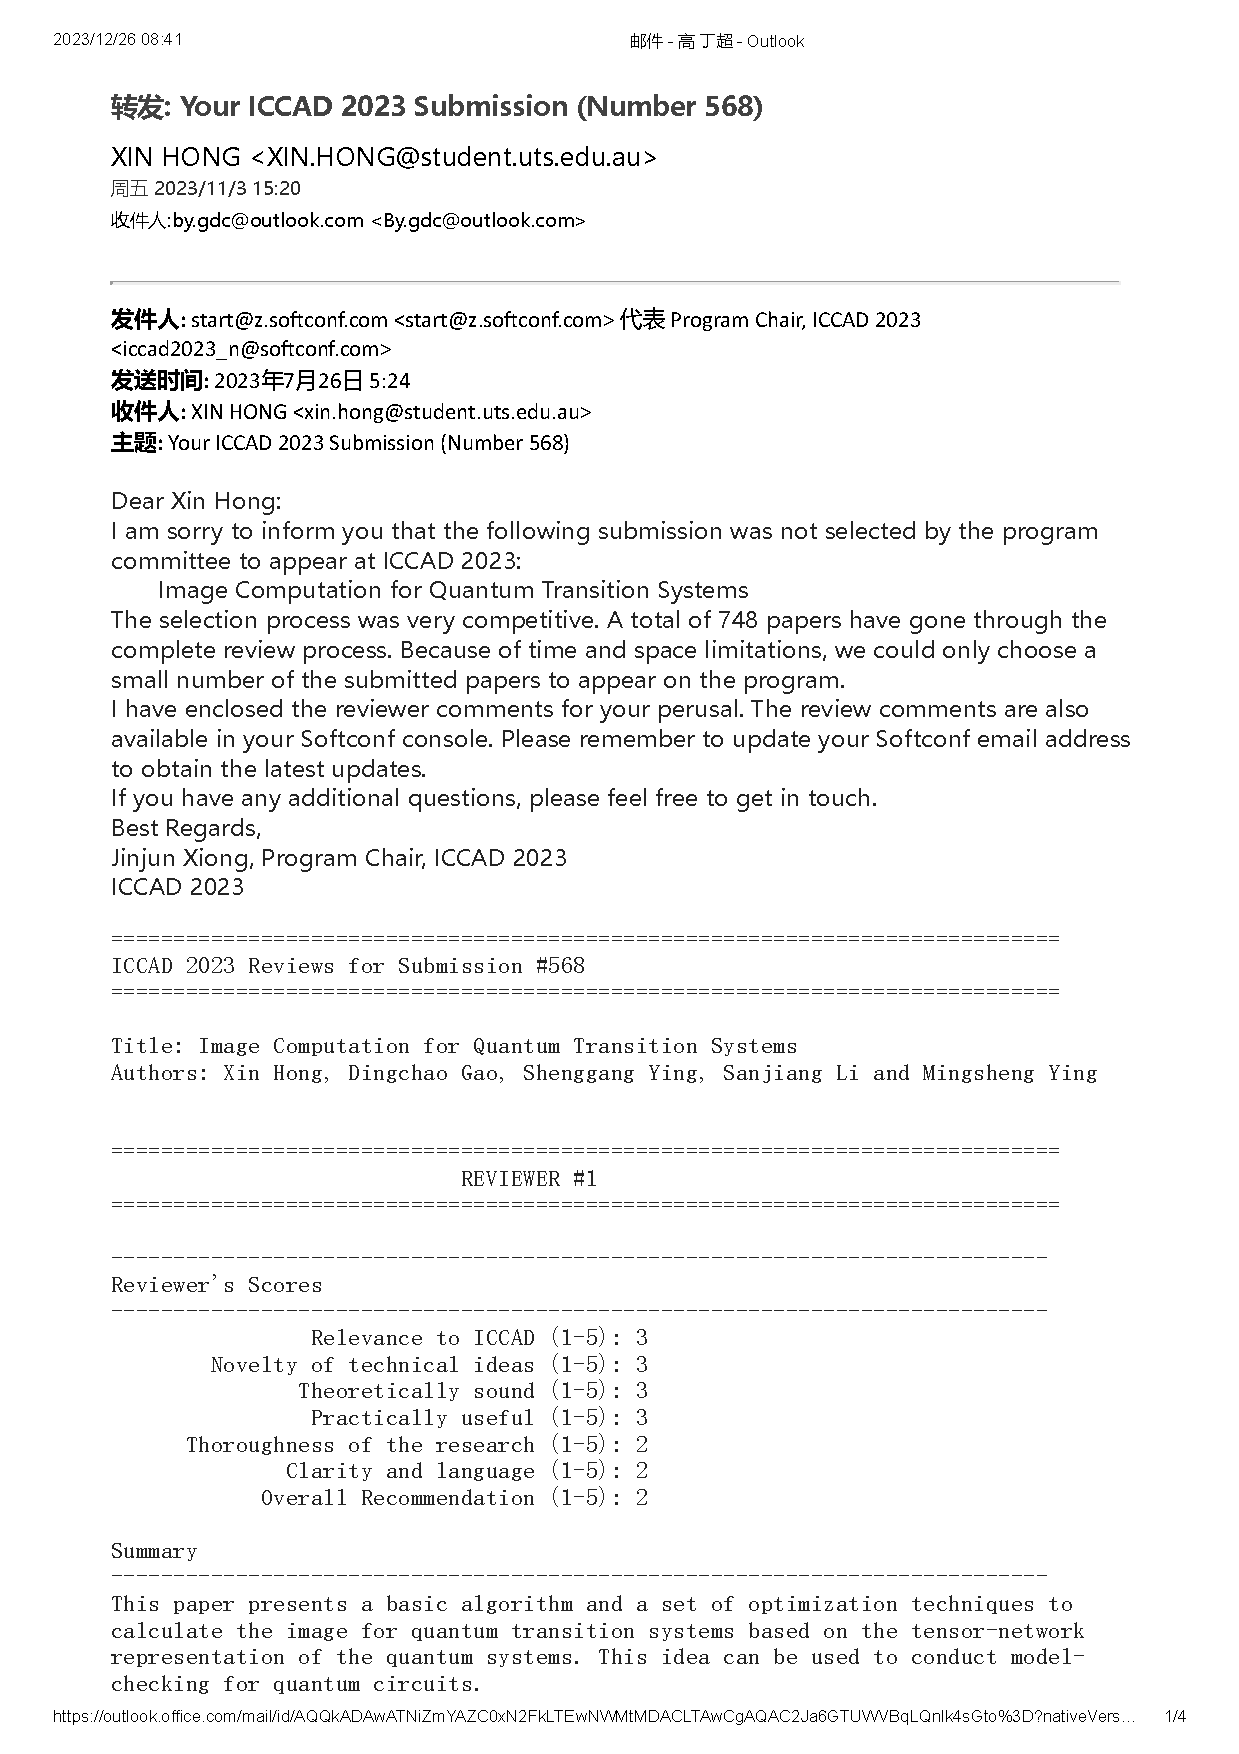
\includepdf[pages=1,scale = 0.8,pagecommand={\section*{附录一ICCAD审稿意见}}]{ICCAD.pdf}
\includepdf[pages=2-,scale = 0.8]{ICCAD.pdf}
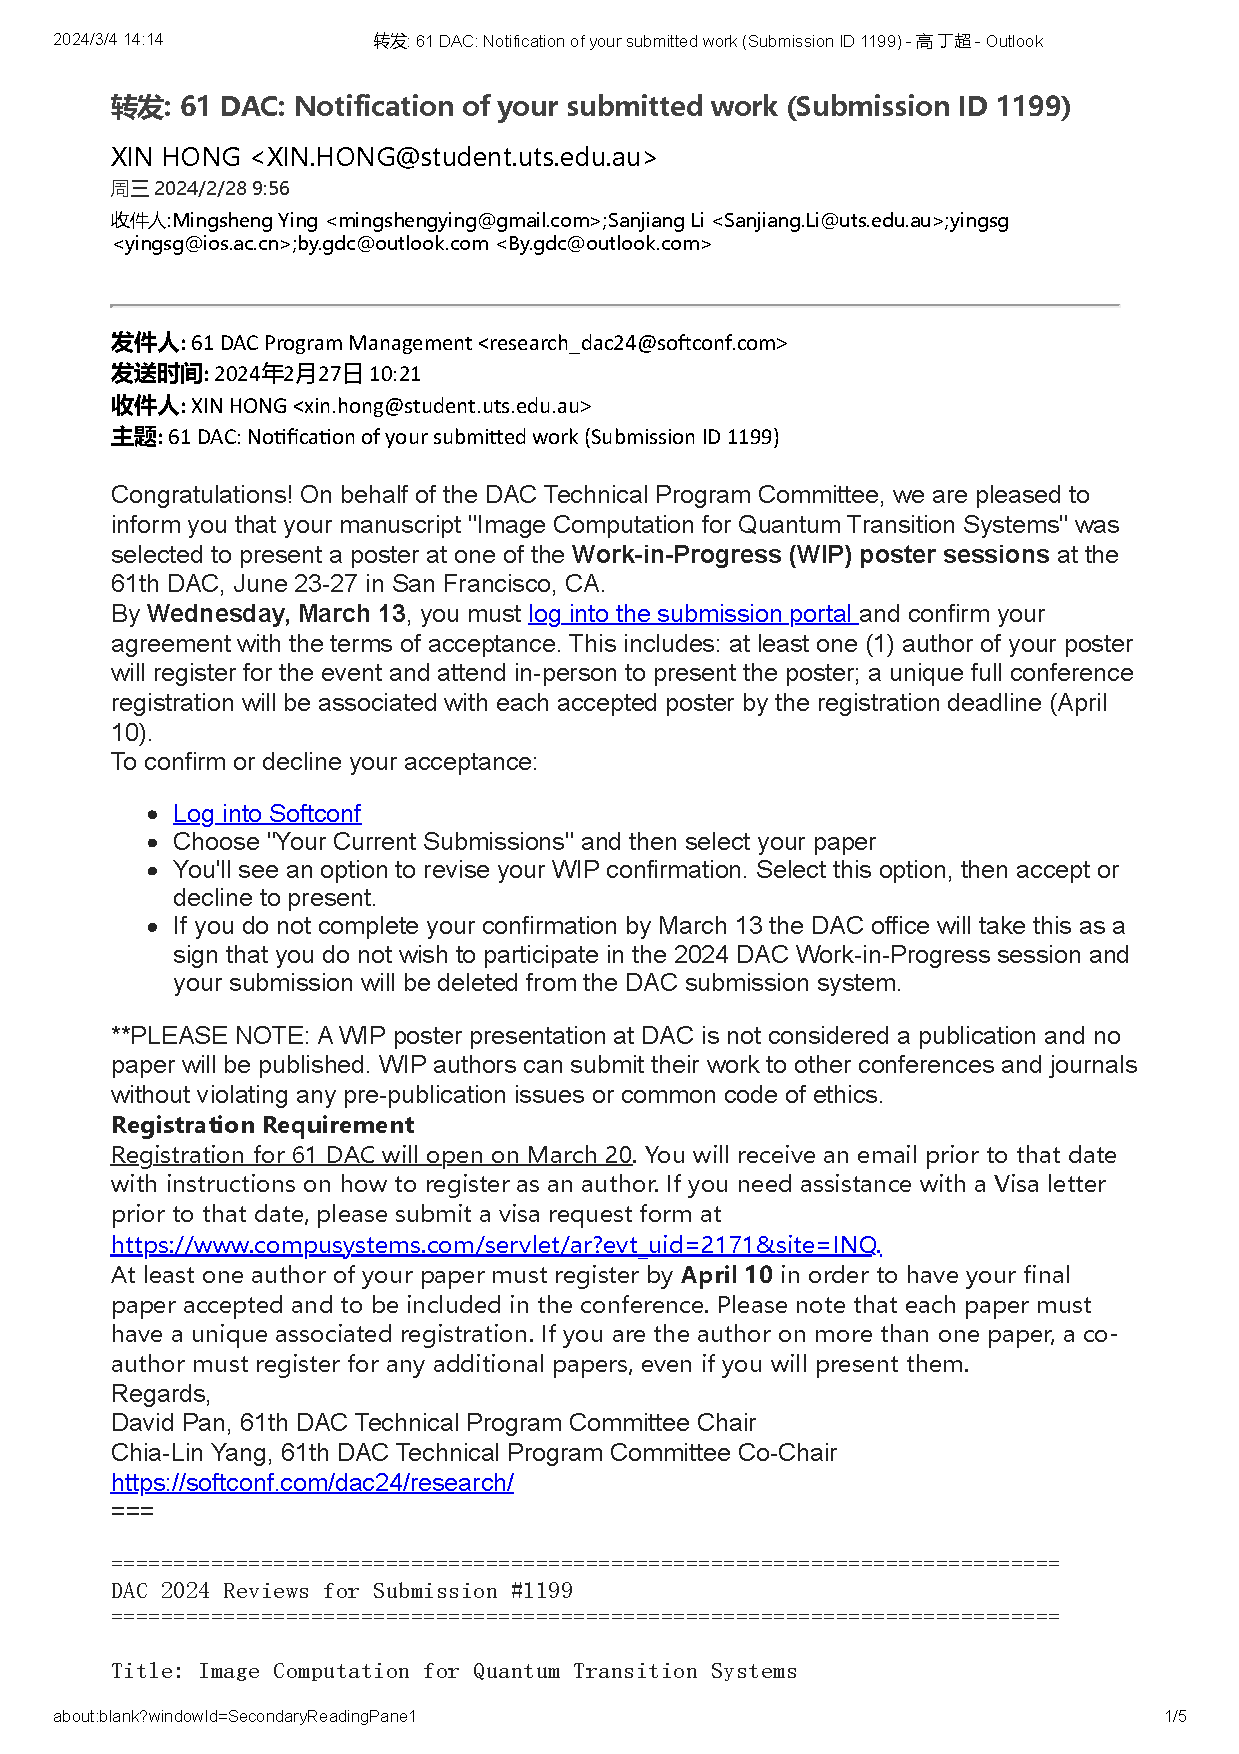
\includepdf[pages=1,scale = 0.8,pagecommand={\section*{附录二DAC审稿意见}}]{DAC.pdf}
\includepdf[pages=2-,scale = 0.8]{DAC.pdf}
\end{document}
